%%%%%%%%%%%%%%%%%%%%%%%%%%%%%%%%%%%%%%%%%%%%%%%%%%%%%%%%%%%%%%%%%
\chapter{MATHEMATICAL MODEL}\label{CH2}
%%%%%%%%%%%%%%%%%%%%%%%%%%%%%%%%%%%%%%%%%%%%%%%%%%%%%%%%%%%%%%%%%
\section{Channel Flow}
In this study, steady viscous incompressible flow of an electrically conducting fluid possessing variable viscosity bounded by two infinite horizontal permeable parallel plates with a distance h in between is considered Fig. ~\ref{fig:systemSchematic}.  A constant magnetic field is uniformly applied perpendicular to the plates along the y – axis. The plates are held at constant temperature. The uniform injection and suction through the lower and upper plates are kept at a constant velocity V along the y direction. The assumptions carried through the study can be summarized as;
\begin{itemize} \item The problem is one-dimensional since the plates are assumed to be infinitely long \item 	The induced magnetic field is neglected when compared with the applied magnetic field, due to inherently small magnetic Reynolds number for magnetic liquids and partially ionized fluids \cite{CramerMagneto} \item 	Electric field and Hall effects, the ion-slip and thermoelectric effects, and the electron pressure gradient are all neglected \cite{SethUnsteady} \item  The flow is assumed to be fully developed and the edge effects are neglected.  \end{itemize}

% For one-column wide figures use
\begin{figure*}
% Use the relevant command to insert your figure file.
% For example, with the graphicx package use
  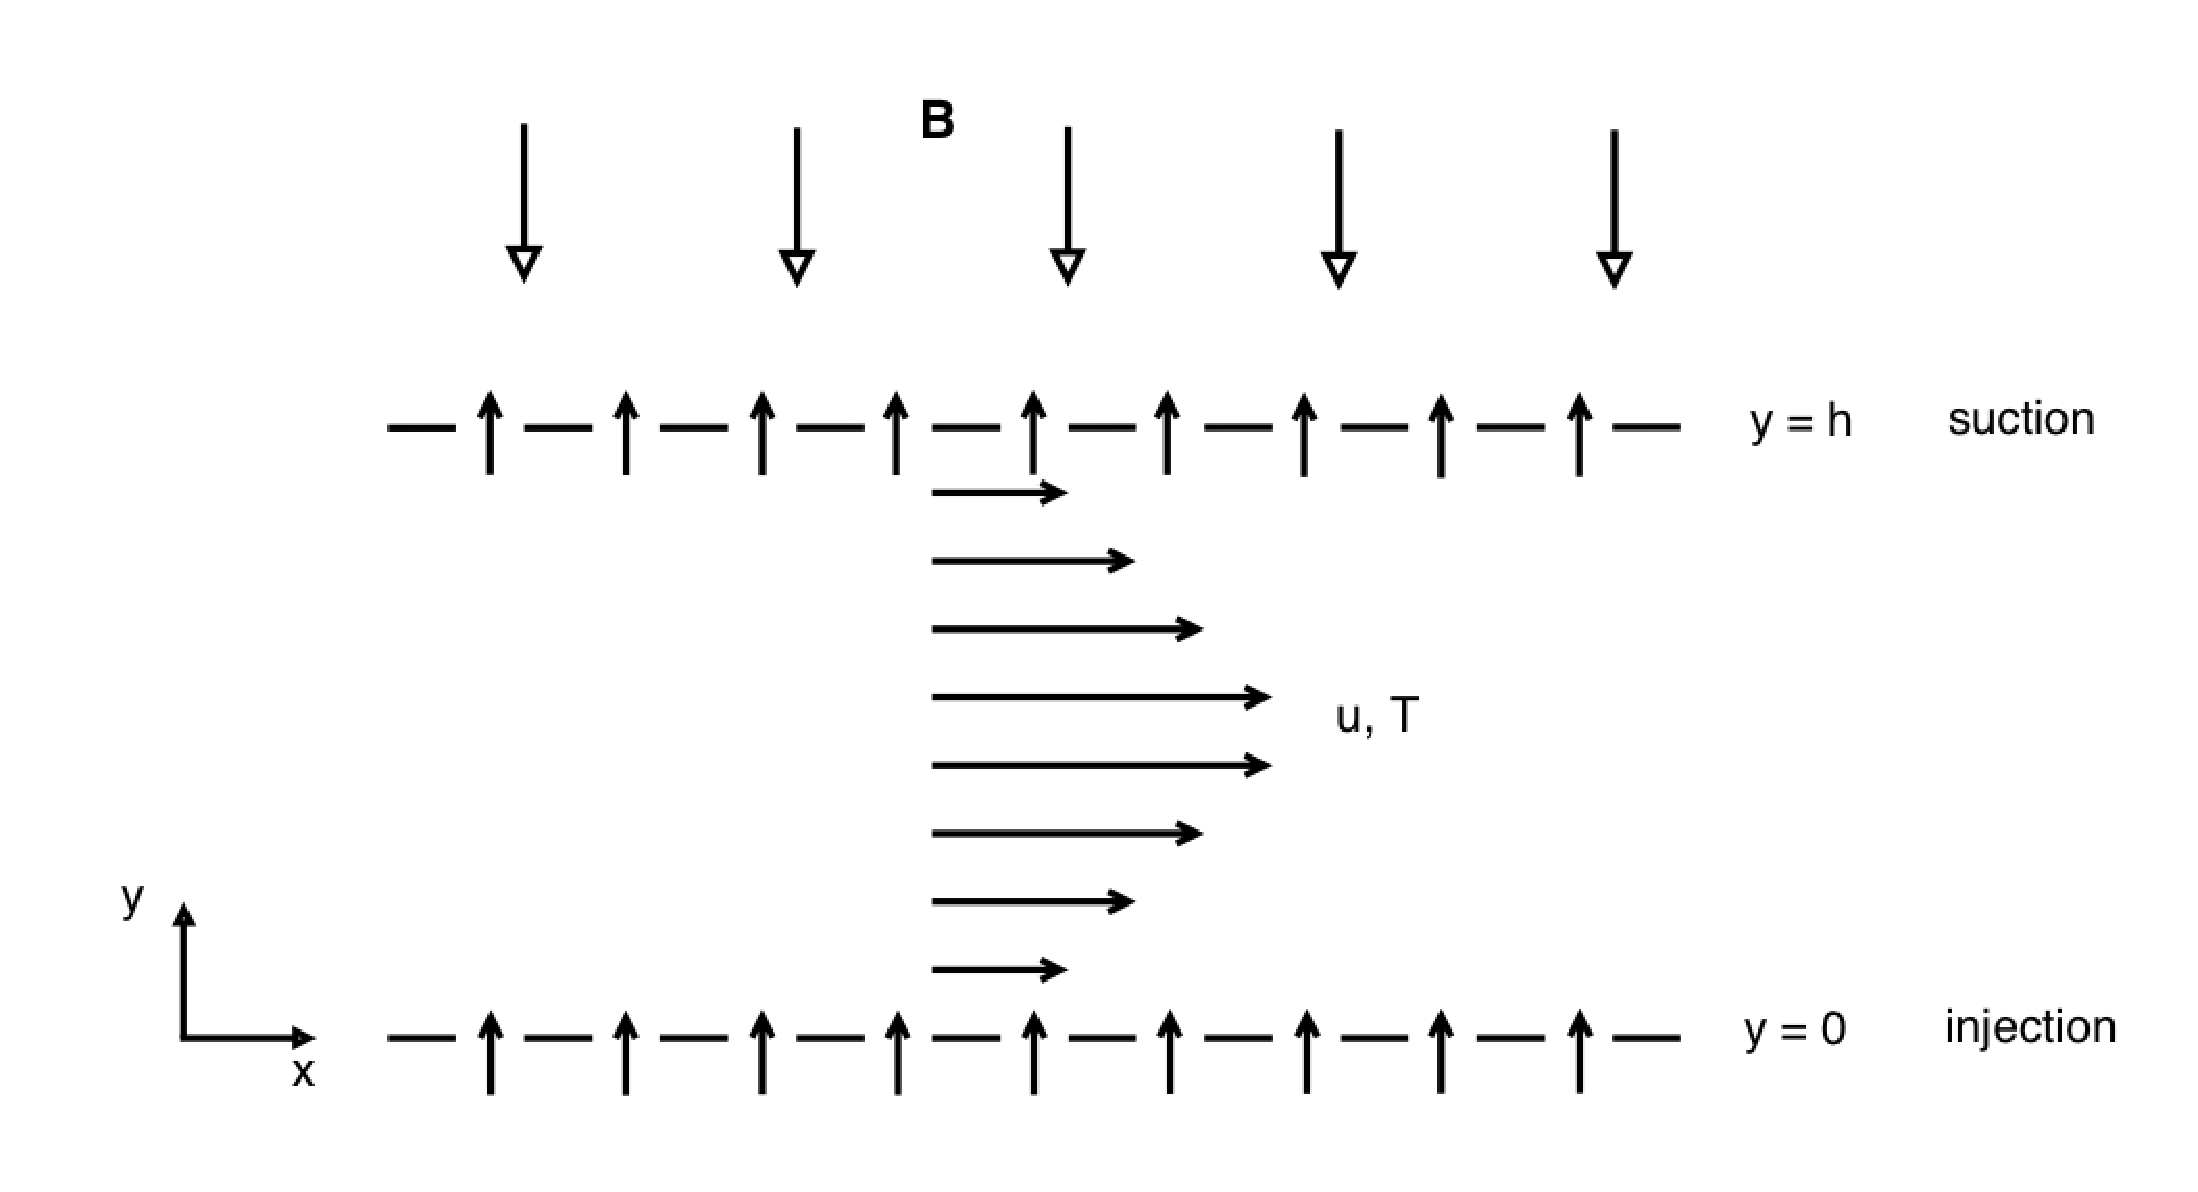
\includegraphics[scale=0.33]{figures/fig1.eps}
% figure caption is below the figure
\vspace*{6mm}
\caption{System Schematic.}
\label{fig:systemSchematic}       % Give a unique label
\end{figure*}

These assumptions enable to write the momentum equation as in \eqref{equ1} for the system given in Fig. ~\ref{fig:systemSchematic}

\begin{equation} \label{equ1}
V\frac{du}{dy}=-\frac{1}{\rho }\frac{\partial p}{\partial x}+\frac{1}{\rho }\frac{d}{dy}\left( \overline{\mu }\left( T \right)\frac{du}{dy} \right)+\frac{{{B}_{0}}}{\rho }{{J}_{z}} 
\end{equation}

where u is the fluid velocity in $x$ direction, $\rho$ is the fluid density, $p$ is the fluid pressure, $V$ is the uniform suction/injection velocity at the channel walls and  ${{J}_{z}}$   is the $z$ dimension of current density vector,  $\overrightarrow{J}$  given by the Ohm'��s Law given in \eqref{densityVector}

\begin{equation} \label{densityVector}
\overrightarrow{J}=\sigma \left[ \overrightarrow{E}+\overrightarrow{q}\times \overrightarrow{B} \right]
\end{equation}

In \eqref{densityVector}, $\overrightarrow{E}$, $\overrightarrow{q}$, $\sigma$ represent the electric field vector, the velocity vector and the electrical conductivity of the fluid respectively. 

The energy equation can be written as in \eqref{energyEquation}

\begin{equation} \label{energyEquation}
V\frac{dT}{dy}=\frac{k}{\rho {{c}_{p}}}\frac{{{d}^{2}}T}{d{{y}^{2}}}+\frac{\overline{\mu }\left( T \right)}{\rho {{c}_{p}}}{{\left( \frac{du}{dy} \right)}^{2}}+\frac{{{J}_{z}}^{2}}{\sigma \rho {{c}_{p}}}
\end{equation}

where $\overline{\mu }$ is the viscosity coefficient,  $k$  is the thermal conductivity coefficient, ${c}_{p}$  is the specific heat at constant pressure,  $T$ is the fluid temperature.
Considering the motion is steady $\Delta \times \overset{\lower0.5em\hbox{$\smash{\scriptscriptstyle\rightharpoonup}$}}{E}=0$, results in
\begin{align}
\frac{d{{E}_{x}}}{dy}&=0   & \frac{d{{E}_{x}}}{dy}&=0
\end{align}
Since ${{E}_{x}}$ and ${{E}_{z}}$ are constants, assuming ${{E}_{x}}={{E}_{z}}=0$ yields
\begin{align}
{{J}_{x}} &=0   & {{J}_{z}}&=-\sigma u{{B}_{0}}
\end{align}

Evaluating these relations in \eqref{equ1}-\eqref{energyEquation}, gives the governing equations as in \eqref{nondimensionalEquationsPorousChannel1}-\eqref{nondimensionalEquationsPorousChannel2} \cite{EegunjobiEntropy,SDas,AgarwalOn}
\begin{align}
V\frac{du}{dy}&=-\frac{1}{\rho }\frac{\partial p}{\partial x}+\frac{1}{\rho }\frac{d}{dy}\left( \overline{\mu }\left( T \right)\frac{du}{dy} \right)-\frac{\sigma {{B}_{0}}^{2}u}{\rho }\label{nondimensionalEquationsPorousChannel1}\\
V\frac{dT}{dy}&=\alpha \frac{{{d}^{2}}T}{d{{y}^{2}}}+\frac{\overline{\mu }\left( T \right)}{\rho {{c}_{p}}}{{\left( \frac{du}{dy} \right)}^{2}}+\frac{\sigma {{B}_{0}}^{2}{{u}^{2}}}{\rho {{c}_{p}}} \label{nondimensionalEquationsPorousChannel2}
\end{align}

where viscosity is given in \eqref{viscosityEqu}
\begin{equation} \label{viscosityEqu}
\bar{\mu }\left( T \right)={{\mu }_{0}}{{e}^{-m\left( T-{{T}_{1}} \right)}}
\end{equation}

$m$ is viscosity variation parameter, ${{\mu }_{0}}$ is the fluid dynamic viscosity at the ambient temperature. The boundary conditions are given in \eqref{equ9}-\eqref{equ10}
\begin{align}
u\left( 0 \right)&=0   & -k\frac{dT}{dy}\left( 0 \right)&={{\gamma }_{0}}\left( {{T}_{1}}-T\left( 0 \right) \right) \label{equ9} \\
u\left( h \right)&=0   & -k\frac{dT}{dy}\left( h \right)&={{\gamma }_{1}}\left( T\left( h \right)-{{T}_{2}} \right) \label{equ10}
\end{align}

where ${{\gamma }_{0}}$ and  ${{\gamma }_{1}}$ are the heat transfer coefficients at the lower and upper plates respectively. ${T}_{1}$ is the temperature of the hot fluid at the lower permeable plate and ${T}_{2}$ is the ambient temperature above the upper plate.

Introducing the non-dimensional variables 

\begin{align}
Y&=\frac{y}{h}\ &  X&=\frac{x}{h}\    & U&=\frac{u}{{{U}_{\infty }}}  & \theta&=\frac{T-{{T}_{2}}}{{{T}_{1}}-{{T}_{2}}} \label{nonDimVarSet1}\\      
\mu &=\frac{\overline{\mu }}{{{\mu }_{0}}} & P&=\frac{ph}{{{\mu }_{0}}{{U}_{\infty }}} & G&=-\frac{\partial P}{\partial X} & {{V}^{*}}&=\frac{V}{{{U}_{\infty }}} \label{nonDimVarSet2}
\end{align}

Although the non-dimensional variables given above is written in advance, it is not a one step approach and the non-dimensionalization is held flawlessly after defining them. It is an iterative process and for some people is even art, since knowledge of the system in question is required. These are the resulted non-dimensionalized variables which enable the non-dimensionalization as explained below. To explain the non-dimensionalization \eqref{nondimensionalEquationsPorousChannel1} and \eqref{nondimensionalEquationsPorousChannel2} will be handled one by one. First calculate the derivatives for the dimensionalized temperature $T$ to substitute with the non-dimensionalized temperature $\theta$ in \eqref{nondimensionalEquationsPorousChannel2}. 

\begin{align}
d\theta &= \frac{dT}{T_1 - T_2}\\
dY &= \frac{dy}{h} 
\end{align}

And dividing and rearranging yields,
\begin{equation} \label{Tderiv1}
\frac{dT}{dy} = \frac{(T_1 - T_2)}{h} \frac{d\theta}{dY}
\end{equation}
 
 And the second derivative
 
\begin{align}
\begin{split}
\frac{d^2T}{dy^2} &= \frac{d}{dy}\left( \frac{dT}{dy} \right) = \frac{1}{h}\frac{d}{dY} \left( \frac{T_1 - T_2}{h} \cdot \frac{d\theta}{dY} \right) \\
 &= \frac{T_1-T_2}{h^2}\frac{d^2\theta}{dY^2} \label{Tderiv2}
 \end{split}
\end{align}

Likewise for the derivative of $u$;

\begin{equation} \label{uderiv}
\frac{du}{dy} =  \frac{U_\infty}{h} \frac{dU}{dY} 
\end{equation}

\eqref{Tderiv1}, \eqref{Tderiv2} and \eqref{uderiv} substituted in \eqref{nondimensionalEquationsPorousChannel2} yields 

\begin{equation} \label{goOnWithNonDim1}
V \frac{T_1-T_2}{h} \frac{d\theta}{dY} = \alpha \frac{T_1-T_2}{h^2} \frac{d^2\theta}{dY^2} + \frac{\overline{\mu}(T)}{\rho c_p} \left( \frac{U_\infty}{h} \frac{dU}{dY} \right)^2 + \frac{\sigma B_0^2 U^2 U_\infty^2}{\rho c_p}
\end{equation}

Multiplying the equation \eqref{goOnWithNonDim1} with $\frac{h^2}{\alpha(T_1-T_2)}$ and using the viscosity definition given in \eqref{viscosityEqu}, 

\begin{align}
\begin{split}
\frac{h^2}{\alpha(T_1-T_2)}\frac{V(T_1-T_2)}{h}\frac{d\theta}{dY} &= \frac{d^2\theta}{dY^2} + \frac{h^2}{\alpha(T_1 - T_2)}\frac{\mu_0 e^{-m(T-T_1)}}{\rho c_p} \frac{U_\infty^2}{h^2} \left( \frac{dU}{dY} \right)^2 \\
&+ \frac{h^2}{\alpha(T_1 - T_2)} \frac{\sigma B_0^2 U_\infty^2}{\rho c_p}  U^2
\end{split}
\end{align}


Introducing Eckart number as in \eqref{EckNum};

\begin{equation} \label{EckNum}
Ec = \frac{U_\infty^2}{c_p (T_1-T_2)} 
\end{equation}

 and rearranging terms and multiply and divide the last term by $\mu_0$ leads to \eqref{equNonDimStep}.

\begin{equation} \label{equNonDimStep}
\frac{d^2\theta}{dY^2} - \frac{hV}{\alpha} \cdot \frac{d\theta}{dY} + \frac{\mu_0 e^{-m(T-T_1)}}{\alpha\rho} \cdot Ec \cdot \left( \frac{dU}{dY}\right)^2 + \frac{B_0^{2}h^{2}\sigma }{\alpha \rho } \cdot \frac{\mu_{0}}{\mu_{0}} \cdot Ec \cdot U^{2} = 0
\end{equation}

Next step is to define $Ha$ number as in Eq. \eqref{HaNumber}.

\begin{equation} \label{HaNumber}
Ha ={{B}_{0}}h\sqrt{\frac{\sigma }{{{\mu }_{0}}}}
\end{equation}

Substituting Ha number in \eqref{equNonDimStep} and manipulating the second term by multiplying and dividing by $U_\infty \cdot V \cdot \alpha \cdot \upsilon$

\begin{align}
\begin{split} \label{equNonDimStep2}
\frac{d^2\theta}{dY^2} - \frac{hV}{\alpha} \cdot \dfrac{U_\infty}{U_\infty} \cdot \frac{V}{V} \cdot \frac{\alpha}{\upsilon} \cdot \frac{\upsilon}{\alpha} \cdot \frac{d\theta}{dY} &+ \frac{\mu_0 e^{-m(T-T_1)}}{\alpha\rho} \cdot Ec \cdot \left( \frac{dU}{dY}\right)^2 \\
&+ \frac{{Ha}^{2} \mu_{0}}{\alpha \rho } \cdot Ec \cdot U^{2} = 0
\end{split}
\end{align}

Introducing Re and Pr number 

\begin{align}
Re &= \frac{U_\infty h}{\upsilon} \label{ReNumber}\\
Pr &= \frac{\upsilon}{\alpha}
\end{align}

and evaluate in \eqref{equNonDimStep2} gives \eqref{equNonDimStep3}.

\begin{equation} \label{equNonDimStep3} 
\frac{d^2\theta}{dY^2} -  Re \cdot Pr \cdot \frac{V}{U_\infty} \cdot \frac{d\theta}{dY} + \frac{\mu_0 e^{-m(T-T_1)}}{\alpha\rho} \cdot Ec \cdot \left( \frac{dU}{dY}\right)^2 +  {Ha}^{2} \cdot Pr \cdot Ec \cdot U^{2}= 0
\end{equation}

For further manipulations, power of the exponential terms has been multiplied and divided by $\epsilon \cdot \theta$

\begin{align}
\begin{split} \label{equNonDimStep4}
\frac{d^2\theta}{dY^2} -  Re \cdot Pr \cdot \frac{V}{U_\infty} \cdot \frac{d\theta}{dY} &+ \frac{\mu_0 e^{-m(T-T_2) \cdot \frac{\varepsilon}{m(T_1-T_2)} \cdot \theta \cdot\frac{(T_1-T_2)}{(T-T_2)} }}{\alpha\rho} \cdot Ec \cdot \left( \frac{dU}{dY}\right)^2 \\
&+  {Ha}^{2} \cdot Pr \cdot Ec \cdot U^{2}= 0
\end{split}
\end{align}

where 

\begin{equation}
\epsilon = m \cdot (T_1 - T_2)
\end{equation}

Rearranging results in the final form of non-dimensionalized equation as in \eqref{equNonDimStep5}

\begin{equation} \label{equNonDimStep5} 
\frac{d^2\theta}{dY^2} - Re \cdot Pr \cdot \frac{V}{U_\infty} \cdot \frac{d\theta}{dY} + Pr \cdot Ec \cdot e^{- \varepsilon \theta} \cdot \left( \frac{dU}{dY}\right)^2 + Ha^{2} \cdot Ec \cdot  Pr \cdot U^{2} = 0
\end{equation}

Since one of the two equations is now non-dimensionalised, Eq.\eqref{nondimensionalEquationsPorousChannel1} will be non-dimensionalised next. For that purpose, Eq. \eqref{viscosityEqu} for viscosity, derivative of velocity from Eq. \eqref{uderiv},  and derivative of pressure is calculated as in  Eq. \eqref{pressureDeriv}


\begin{equation}\label{pressureDeriv}
dP = \frac{dp \cdot h}{{{\mu }_{0}}{{U}_{\infty }}}
\end{equation}

and substituted in Eq.\eqref{nondimensionalEquationsPorousChannel1} gives

\begin{equation}
V \frac{U_\infty}{h}\frac{dU}{dy} = - \frac{1}{\rho} \cdot \frac{\mu_{0}U_\infty}{h^{2}} \cdot \frac{dP}{dX}  + \frac{\mu_{0}}{\rho} \cdot \frac{d}{dy} \left( e^{-m(T-T_2)} \cdot \frac{du}{dy} \right) - \frac{\sigma B_0^{2}U_\infty}{\rho}U
\end{equation}

taking the derivative of the second term in the right side of the equation gives

\begin{align}
\begin{split} \label{equNonDimSecondEqStep1}
V \frac{U_\infty}{h}\frac{dU}{dY} = &- \frac{1}{\rho} \cdot \frac{\mu_{0}U_\infty}{h^{2}} \cdot \frac{dP}{dX}  + \frac{\mu_{0}}{\rho} \left[ -mT e^{-m(T-T_2)} \frac{dT}{dy}\frac{du}{dy} + e^{-m(T-T_2)}\frac{d^{2}u}{dy^{2}} \right] \\
&- \frac{\sigma B_0^{2}U_\infty}{\rho}U
\end{split}
\end{align}

Now substituting Eq. \eqref{Tderiv1} and Eq. \eqref{uderiv} in  Eq. \eqref{equNonDimSecondEqStep1}

\begin{align}
\begin{split} \label{equNonDimSecondEqStep2}
V \frac{U_\infty}{h}\frac{dU}{dY} = &- \frac{1}{\rho} \cdot \frac{\mu_{0}U_\infty}{h^{2}} \cdot \frac{dP}{dX}  \\
 \displaystyle &+ \frac{\mu_{0}}{\rho} \left[ -m e^{-m(T-T_2)} \frac{(T_1-T_2)}{h} \frac{U_\infty}{h}\frac{d\theta}{dY}\frac{dU}{dY} + e^{-m(T-T_2)}\frac{U_\infty}{h^{2}}\frac{d^{2}U}{dY^{2}} \right]  \\
 &- \frac{\sigma B_0^{2}U_\infty}{\rho}U
\end{split}
\end{align}

Dividing the equation with $\frac{\mu_{0}}{\rho}\frac{U_\infty}{h^{2}}e^{-m(T-T_2)}$ and substituting for Ha number given in Eq. \eqref{HaNumber}

\begin{align}
\begin{split} \label{equNonDimSecondEqStep3}
\frac{d^{2}U}{dY^{2}} &- e^{m(T-T_2)} \frac{V} {U_\infty} U_\infty \frac{\rho}{\mu_{0}} h \frac{dU}{dY} 
- e^{m(T-T_2)} \frac{dP}{dX} \\
&- m(T_1-T_2)\frac{d\theta}{dY}\frac{dU}{dY} 
- Ha^{2}e^{m(T-T_2)} U = 0
\end{split}
\end{align}

Substituting Re number from Eq. \eqref{ReNumber} and nondimensionalized temperature in the exponential term 

\begin{align}
\begin{split} \label{equNonDimSecondEqStep4}
\frac{d^{2}U}{dY^{2}} &- e^{m(T-T_2)\varepsilon \frac{1}{m(T_1-T_2)}\theta\frac{(T_1-T_2)}{(T-T_2)}} 
\frac{V} {U_\infty} Re \frac{dU}{dY} 
- e^{m(T-T_2)} \frac{dP}{dX} \\
&- \varepsilon\frac{d\theta}{dY}\frac{dU}{dY} - e^{\varepsilon\theta}Ha^{2} U = 0
\end{split}
\end{align}

Finally rearranging gives the nondimensionalized form of Eq.\eqref{nondimensionalEquationsPorousChannel1} 

\begin{equation}
\frac{d^{2}U}{dY^{2}} - e^{\varepsilon\theta} \left[ \frac{V} {U_\infty} Re \frac{dU}{dY} + \frac{dP}{dX} + Ha^{2} U \right] - \varepsilon \frac{d\theta}{dY}\frac{dU}{dY} = 0
\end{equation}
 
So non-dimensional governing equations in summary can be written as

\begin{align}
 \frac{{{d}^{2}}U}{d{{Y}^{2}}}-\varepsilon \frac{d\theta }{dY}\frac{\partial U}{\partial Y}-{{e}^{\varepsilon \theta }}\left( {{V}^{*}}\operatorname{Re}\frac{dU}{dY}+H{{a}^{2}}U-G \right)&=0 \label{nonDimEquOfSystem1}\\
\frac{{{d}^{2}}\theta }{d{{Y}^{2}}}-{{V}^{*}}\operatorname{Re}\Pr \frac{d\theta }{dY}+Br{{e}^{-\varepsilon \theta }}{{\left( \frac{dU}{dY} \right)}^{2}}+BrH{{a}^{2}}{{U}^{2}}&=0\ \label{nonDimEquOfSystem2}
\end{align}

where

\begin{align}
\operatorname{Re}&=\frac{{{U}_{\infty }}h}{\upsilon } &  \Pr &=\frac{\upsilon }{\alpha }    &  Ec&=\frac{U_{\infty }^{2}}{{{c}_{p}}\left( {{T}_{1}}-{{T}_{2}} \right)} \label{equNonDimParameters1} \\ Br&=Ec\cdot \Pr   & Ha&={{B}_{0}}h\sqrt{\frac{\sigma }{{{\mu }_{0}}}} & \varepsilon &=m\left( {{T}_{1}}-{{T}_{2}} \right) \label{equNonDimParameters2} \\ 
B{{i}_{0}}&=\frac{{{\gamma }_{0}}h}{k} & B{{i}_{1}}&=\frac{{{\gamma }_{1}}h}{k} & V^* &= \frac{V}{U_\infty} \label{equNonDimParameters3}
\end{align}

The non-dimensionalized governing equations given in \eqref{nonDimEquOfSystem1}-\eqref{nonDimEquOfSystem2} are subject to boundary conditions below

\begin{align}
U\left( 0 \right)&=0   & \frac{d\theta }{dY}\left( 0 \right)&=B{{i}_{0}}\left( \theta \left( 0 \right)-1 \right)  \label{equ18} \\
U\left( 1 \right)&=0   & \frac{d\theta }{dY}\left( 1 \right)&=-B{{i}_{1}}\theta \left( 1 \right) \label{equ19}
\end{align}

The governing equations given in \eqref{nonDimEquOfSystem1}-\eqref{nonDimEquOfSystem2} and the boundary conditions including partial derivatives in \eqref{equ18}-\eqref{equ19} are discretized utilizing GDQM. Then the resulting system of algebraic equations is solved by Newton-Raphson Algorithm.

\section{Entropy Generation}
\label{sec:3}
Designing optimal engineering systems is a key goal in energy efficiency \cite{heatTransSecLaw1,heatTransSecLaw2}. To predict the performance of the processes, second law of thermodynamics has been applied for years. However, Bejan introduced the idea of entropy generation minimization to optimize heat exchange system. 
The convection process in a channel is inherently irreversible which causes entropy generation. Local volumetric entropy generation rate formula for a viscous incompressible conducting fluid in the presence of magnetic field is given by \cite{WoodsThermo} as \eqref{localEntropyGeneration}, indicating each terms irreversibility reason

\begin{equation} \label{localEntropyGeneration}
{{E}_{G}}=\underbrace{\frac{k}{T_{2}^{2}}{{\left( \frac{dT}{dy} \right)}^{2}}}_{heat\_transfer}+\underbrace{\frac{\mu }{{{T}_{2}}}{{\left( \frac{du}{dy} \right)}^{2}}}_{viscous\_dissipation}+\underbrace{\frac{\sigma B_{0}^{2}}{{{T}_{2}}}{{u}^{2}}}_{magnetic\_field}
\end{equation}

The last term in the right side of \eqref{localEntropyGeneration} is the entropy generation due to magnetic field. Evaluating non-dimensional parameters given in \eqref{nonDimVarSet1}-\eqref{nonDimVarSet2}, \eqref{equNonDimParameters1} - ��\eqref{equNonDimParameters3}, local entropy generation rate is defined as in \eqref{localEntropyGenerationRate}.

 \begin{equation} \label{localEntropyGenerationRate}
{{N}_{S}}=\frac{T_{2}^{2}{{h}^{2}}{{E}_{G}}}{k{{\left( {{T}_{1}}-{{T}_{2}} \right)}^{2}}}={{\left( \frac{d\theta }{dY} \right)}^{2}}+\frac{Br}{\Omega }\left( {{e}^{-\varepsilon \theta }}{{\left( \frac{dU}{dY} \right)}^{2}}+Ha{{U}^{2}} \right)
\end{equation}

Here $\Omega $ and $Br$ stand for the temperature difference parameter and Brinkmann number respectively and can be given as $\Omega =\frac{\left( {{T}_{1}}-{{T}_{2}} \right)}{{{T}_{2}}}$, $Br=Ec\Pr $. To show the dominance of irreversibility due to heat transfer with respect to the combined effect of fluid friction and magnetic fields, Bejan number is introduced as follows

\begin{equation} \label{equ27}
Be=\frac{{{N}_{heat}}}{{{N}_{S}}}=\frac{{{\left( \frac{d\theta }{dY} \right)}^{2}}}{{{\left( \frac{d\theta }{dY} \right)}^{2}}+\frac{Br}{\Omega }\left( {{e}^{-\varepsilon \theta }}{{\left( \frac{dU}{dY} \right)}^{2}}+Ha{{U}^{2}} \right)}
\end{equation}

$Be$ number ranges between 0 and 1 with a meaning of dominance of irreversibility due to heat transfer dominates for the values closer to 1, and the combination of fluid friction and magnetic field for the values closer to 0. 

\section{Nanofluid Channel Flow}

In this study, steady viscous incompressible flow of a Cu - Water nanofluid  bounded by two infinite horizontal parallel plates with a distance $H$ in between is considered. Cartesian coordinate axes are selected as reference, $x$ � axis parallel to plates and located at the same distance to the plates, y - axis along the direction perpendicular to the plates as can be seen in Fig.~\ref{sysConfigNano}.  A constant magnetic field  is applied perpendicular to the plates uniformly along y � axis. The plates are sustained to have a constant temperature of ${{T}_{{{w}_{2}}}}$  and  ${{T}_{{{w}_{1}}}}$, at the lower and upper plates respectively. The assumptions carried through the study can be summarized as;

\begin{figure}[t]
\begin{center}
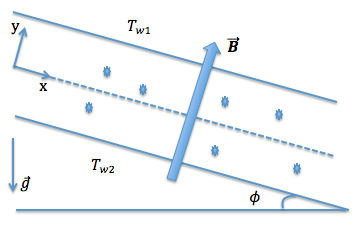
\includegraphics[scale=0.7]{figures/systemConfigxyOrtada.png}
\end{center}
\vspace*{6mm}
\caption{Schematic configuration of the problem.}
\label{sysConfigNano} 
\end{figure}

\begin{itemize} \item The plates are infinitely long, enabling to consider the problem one dimensional. \item The induced magnetic field is neglected when compared with the applied magnetic field , due to inherently small magnetic Reynolds number for magnetic liquids and partially ionized fluids \cite{MHDbook}. \item 	Electric field and Hall effects, the ion-slip and thermoelectric effects, and the electron pressure gradient are neglected \cite{unsteadyCouette,EntGenVarViscosityMHDChannel}. \item  The flow is assumed to be fully developed and the edge effects are neglected.  
The schematic configuration of the considered system is given in Figure~\ref{sysConfigNano}. The inclined channel filled with nanofluids is exposed to magnetic field ${{B}_{0}}$. Under these assumptions the nonlinear coupled differential equations governing the system is given in \eqref{nanofluidChannel1} - \eqref{nanofluidChannel2}.  \end{itemize}

\begin{align}
{{\mu }_{nf}}\frac{{d^{2}}u}{d{{y}^{2}}}+{{\left( \rho \beta  \right)}_{nf}}g\sin \phi \left( T-{{T}_{w2}} \right)-{{\sigma }_{nf}}B_{0}^{2}u&=\frac{dp}{dx} \label{nanofluidChannel1}\\
\frac{{{d}^{2}}T}{d {{y}^{2}}}+\frac{{{\mu }_{nf}}}{{{k}_{nf}}}{{\left( \frac{du}{dy} \right)}^{2}}+\frac{{{\sigma }_{nf}}}{{{k}_{nf}}}B_{0}^{2}{{u}^{2}}&=0 \label{nanofluidChannel2}\
% hic bir sey yazmazsan esitlikleri alt alta hizaliyor canim benim&=alo \\
% $ tek dolar arasi $ inline denklem
% $$ cift dolar arasi $$ satir atlayarak ortada denklem
\end{align}
The system of equations in \eqref{nanofluidChannel1} - \eqref{nanofluidChannel2} is subject to boundary conditions given in \eqref{nanofluidChannelBoundary1} - \eqref{nanofluidChannelBoundary2}
\begin{align}
u(H / 2)&=0   & u(-H / 2)&=0 \label{nanofluidChannelBoundary1}\\
T(H / 2)&= {T}_{w1} & T(- H / 2)&= {T}_{w2} \label{nanofluidChannelBoundary2}
\end{align}
Addition of nanoparticles changes the thermophysical properties of the fluid flow. There are numerous work to model the surprising nature of the nanofluids but there is no consensus yet. Available models depend on different parameters, e.g the nanoparticle material, the volume fraction of nanofluids, specific heat, and others. In this study, the thermal conductivity model for the nanofluids given in Eq. \eqref{thermalCondChoi} is presented by Choi \cite{ChoiNanofluidThermalCond}, Brinkmann model \cite{BrinkmannModelViscosity} given in Eq. \eqref{viscosityBrinkmann} for nanofluid viscosity. The temperature dependency of these parameters given in Eqs. \eqref{alphaNanofluid}-\eqref{viscosityBrinkmann} are ignored as usual in the literature investigating nanofluid flows, but should be considered in the following research.
\begin{align}
{{\alpha }_{f}} &=\frac{{{k}_{f}}}{{{\left( \rho {{c}_{p}} \right)}_{f}}} \label{alphaNanofluid}\\
{{\rho }_{nf}} &=\left( 1-\psi  \right){{\rho }_{f}}+\psi {{\rho }_{p}} \label{rhoNanofluid}\\     
\frac{{{k}_{nf}}}{{{k}_{f}}}&=\frac{{{k}_{p}}+2{{k}_{f}}-2\psi \left( {{k}_{f}}-{{k}_{p}} \right)}{{{k}_{p}}+2{{k}_{f}}+2\psi \left( {{k}_{f}}-{{k}_{p}} \right)} \label{thermalCondChoi}\\   
\frac{{{\mu }_{nf}}}{{{\mu }_{f}}}&=\frac{1}{{{\left( 1-\psi  \right)}^{2.5}}} \label{viscosityBrinkmann}
\end{align}

To derive the dimensionless forms of the governing equations, the following parameters in \eqref{yxNonDim}-\eqref{PNonDim} are defined.

\begin{align}
Y&=\frac{y}{h}\          &  X&=\frac{x}{h} \label{yxNonDim}  \\
U  &    =\frac{uH}{{{\alpha }_{f}}}\     &       \theta& =\frac{T-{{T}_{w1}}}{{{T}_{w2}}-{{T}_{w1}}} \label{velTempNonDim}\\      
P&=\frac{{{H}^{3}}}{\alpha _{f}^{2}{{\rho }_{nf}}}\left( -\frac{dp}{dx} \right) \label{PNonDim}
\end{align}

% \displaystyle \theta = \frac{T-T_c}{T_H-T_c}
Dimensionalized velocity as a function of non-dimensionalized velocity as given in \eqref{velTempNonDim} is derived once and twice yields to \eqref{derivFirstU} and \eqref{derivSecondU} respectively.

\begin{align}
\frac{du}{dy} &= \frac{\alpha_f}{H^2} \cdot \frac{dU}{dY} \label{derivFirstU}\\
\frac{d^2u}{dy^2} &= \frac{\alpha_f}{H^3} \cdot \frac{d^2U}{dY^2} \label{derivSecondU}
\end{align}

Substituting the non-dimensionalized equals of first and second derivatives in the system equations  \eqref{nanofluidChannel1} - \eqref{nanofluidChannel2} yields

 \begin{equation}
\frac{\alpha_{f}}{H^{3}} \cdot P + \mu_{nf} \cdot \frac{\alpha_{f}}{H^{3}} \cdot \frac{d^{2} U}{dY^{2}} + (\rho\beta)_{nf} g \sin\phi ({{T}_{w2}}-{{T}_{w1}}}) \theta - \sigma_{nf} \beta_{0}^{2} \frac{\alpha_{f}}{H} U = 0
\end{equation}

Multiplying with $\frac{H^{3}}{\alpha_{f}^{2}\rho_{nf}}$ results, equation becomes

\begin{equation}
P + \frac{\mu_{nf}}{\alpha_{f} \rho_{nf}} \cdot \frac{d^{2} U}{dY^{2}}  + (\rho\beta)_{nf} g \sin\phi ({{T}_{w2}}-{{T}_{w1}}}) \theta \frac{H^{3}}{\alpha_{f}^{2} \rho_{nf}} - \frac{\sigma_{nf} H^{2}}{\alpha_{f}\rho_{nf}} \beta_{0}^{2} U = 0 \label{equOnTheWay}
\end{equation}

Defining the non-dimensional variables $Ra$ and $Ha$

\begin{align}
Ra &= \frac{g \beta_{f} H^{3} ({{T}_{w2}}-{{T}_{w1}})}{\upsilon_{f}\alpha_{f}} \label{}\\
Ha &= B_{0} H  \sqrt{\frac{\sigma_{nf}}{\rho_{nf}\upsilon_{f}}}\end{align}

and multiplying and dividing some of the terms of \eqref{equOnTheWay} with $\mu_f$ and $\upsilon_f$ to substitute with $Ra$ and $Ha$ in the equation

 \begin{equation}
 P + \frac{\mu_{nf}}{\alpha_{f} \rho_{nf}} \cdot \frac{d^{2} U}{dY^{2}}  +\frac{ (\rho\beta)_{nf} g \sin\phi ({{T}_{w2}}-{{T}_{w1}}) \theta}{\alpha_{f} \rho_{nf} \alpha_{f}} \cdot \frac{\beta_{f}}{\beta_{f}} \cdot \frac{\nu_{f}}{\nu_{f}} -  \frac{\sigma_{nf} H^{2}\beta_{0}^{2}}{\rho_{nf} \alpha_{f}} \cdot U \cdot \frac{\nu_{f}}{\nu_{f}} = 0
\end{equation}

Replacing the defined $Ra$ and $Ha$ in 

 \begin{equation}
 P + \frac{\mu_{nf}}{\alpha_{f} \rho_{nf}} \cdot \frac{d^{2} U}{dY^{2}}  +\frac{ (\rho\beta)_{nf} g \sin\phi Ra Pr \theta}{\rho_{nf} \beta_{f}} - Pr \cdot Ha^{2} \cdot U = 0\label{nonDimNanoChannel1}
\end{equation}

Thus finally \eqref{nonDimNanoChannel1} is derived from the original dimensionalized equation \eqref{nanofluidChannel1}. So now, non-dimensionalization of \eqref{nanofluidChannel2} will be shown. 

First, the second derivative of the temperature as a function of non-dimensionalized temperature is calculated using \eqref{velTempNonDim},
 
 % I do not know why this is here so just leave it a second:
%\begin{equation}
%\frac{\partial^{2} U}{\partial y^{2}} + \frac{\mu_{nf}}{k_{nf}} \left( \frac{\partial U}{\partial y} \right) ^{2} + \frac{\sigma_{nf}}{k_{nf}} \beta_{0}^{2} U^{2}
%\end{equation}

\begin{equation}
\frac{d^{2} T}{dy^{2}} =  \frac{({{T}_{w2}}-{{T}_{w1}})}{H^{2}} \cdot \frac{d^{2} \theta}{dY^{2}}
\end{equation}

Substituting the states with their non-dimensionalized forms in \eqref{nanofluidChannel2} gives

\begin{equation}
\frac{({{T}_{w2}}-{{T}_{w1}})}{H^{2}} \cdot \frac{d^{2} \theta}{dy^{2}} + \frac{\mu_{nf}}{k_{nf}} \left[ \frac{\alpha_{f}}{H} \cdot dU \cdot \frac{1}{H dY} \right] ^{2} + \frac{\sigma_{nf}}{k_{nf}} \cdot \beta_{0}^{2} \cdot \frac{\alpha_{f}^{2}}{H^{2}} \cdot U^{2} = 0
\end{equation}

Rearranging the terms,

\begin{equation}
\frac{({{T}_{w2}}-{{T}_{w1}})}{H^{2}} \cdot \frac{d^{2} \theta}{dy^{2}} + \frac{\mu_{nf}}{k_{nf}} \cdot \frac{\alpha_{f}^{2}}{H^{4}} \cdot \left( \frac{dU}{dY} \right)^2 + \frac{\sigma_{nf}}{k_{nf}} \cdot \beta_{0}^{2} \cdot \frac{\alpha_{f}^{2}}{H^{2}} \cdot U^{2} = 0
\end{equation}

Multiplying with $\frac{H^{2}}{({{T}_{w2}}-{{T}_{w1}})}$ results, equation becomes

 \begin{equation}
\frac{d^{2} \theta}{dy^{2}} + \frac{\mu_{nf}\alpha_{f}^{2}}{k_{nf} H^{2} ({{T}_{w2}}-{{T}_{w1}})} \cdot \left( \frac{dU}{dY} \right)^2 +  \frac{\sigma_{nf}}{k_{nf}} \cdot \beta_{0}^{2} \cdot \frac{\alpha_{f}^{2}}{({{T}_{w2}}-{{T}_{w1}})} \cdot U^{2} = 0 \label{equOnTheWay2}
\end{equation}

Defining the non-dimensional variables $Ec$, $Pr$ and $Br$

\begin{align}
Ec &= \frac{\alpha_{f}^{2}}{H^{2} {c_{p}}_{f} ({{T}_{w2}}-{{T}_{w1}})} \\
Pr &=  \frac{\mu_{f} {c_{p}}_{f}}{k_{f}} \\
Br &= Ec \cdot Pr = \frac{\alpha_{f}^{2} \mu_{f}}{H^{2} ({{T}_{w2}}-{{T}_{w1}}) k_{f}}
\end{align}

and multiplying and dividing some of the terms of \eqref{equOnTheWay2} with $\mu_{f}$, ${k_{f}$, $\mu_{nf}$, $H^2$, $\rho_{nf}$, $\upsilon_{nf}$ to substitute with $Ec$ and $Pr$, $Br$ and $Ha$ in the equation

\begin{align}
\begin{split}
 \frac{d^{2} \theta}{dy^{2}} &+ \frac{\alpha_{f}^{2}}{H^{2} ({{T}_{w2}}-{{T}_{w1}})} \cdot \frac{\mu_{f}}{k_{f}} \cdot \frac{k_{f}}{\mu_{f}} \cdot \frac{\mu_{nf}}{k_{nf}} \cdot \left( \frac{dU}{dY} \right)^2 \\
 &+ \frac{\sigma_{nf}}{k_{nf}} \cdot \frac{\alpha_{f}^{2}}{({{T}_{w2}}-{{T}_{w1}})} \cdot \beta_{0}^{2} 
 \cdot U^{2} \frac{H^{2}}{H^{2}} \cdot \frac{\rho_{nf}}{\rho_{nf}} \cdot \frac{\upsilon_{nf}}{\upsilon_{nf}} = 0
 \end{split}
\end{align}

Replacing the defined $Br$ and $Ha$ in 

 \begin{equation}
 \frac{d^{2} \theta}{dy^{2}} + Br \cdot \frac{k_{f}}{k_{nf}} \cdot \frac{\mu_{nf}}{\mu_{f}}\cdot \left( \frac{dU}{dY} \right)^2 + \frac{\alpha_{f}^{2} \rho_{nf} \upsilon_{f}}{k_{nf} H^{2} ({{T}_{w2}}-{{T}_{w1}})} \cdot Ha^{2} \cdot U^{2} \cdot \frac{\mu_{f}}{\mu_{f}} \cdot \frac{k_{f}}{k_{f}} = 0
\end{equation}

and rearranging gives

 \begin{equation}
 \frac{d^{2} \theta}{dy^{2}} + \frac{k_{f}}{k_{nf}} \cdot \frac{\mu_{nf}}{\mu_{f}}\cdot Br \cdot \left( \frac{dU}{dY} \right)^2 + \frac{\rho_{nf}}{\rho_{f}} \cdot \frac{k_{f}}{k_{nf}} \cdot Br \cdot Ha^{2} \cdot U^{2} = 0
\end{equation}

To sum up, considering the dimensionless parameters the non-dimensionalized differential equations describing the flow is given in Eq. \eqref{finalNondim1}-\eqref{finalNondim2}
\begin{align}
\frac{{{\mu }_{nf}}}{{{\rho }_{nf}}{{\alpha }_{f}}}\frac{{d^{2}}U}{d{{Y}^{2}}}+\frac{{{\left( \rho \beta  \right)}_{nf}}}{{{\rho }_{nf}}{{\beta }_{f}}}\sin \phi Ra\Pr \theta -\Pr H{{a}^{2}}U+P&=0 \label{finalNondim1}\\
\frac{{{d}^{2}}\theta }{d{{Y}^{2}}}+\frac{{{k}_{f}}{{\mu }_{nf}}}{{{k}_{nf}}{{\mu }_{f}}}Br{{\left( \frac{dU}{dY} \right)}^{2}}+\frac{{{\rho }_{nf}}{{k}_{f}}}{{{\rho }_{f}}{{k}_{nf}}}BrH{{a}^{2}}{{U}^{2}}&=0 \label{finalNondim2}\
% hic bir sey yazmazsan esitlikleri alt alta hizaliyor canim benim&=alo \\
% $ tek dolar arasi $ inline denklem
% $$ cift dolar arasi $$ satir atlayarak ortada denklem
\end{align}

and dimensionless parameters describing characteristics of the fluid flow utilized in dimensionalization  are summarized in Eq. \eqref{nonDimParametersNano1}-\eqref{nonDimParametersNano3}
\begin{align}
Ha& ={{B}_{0}}H\sqrt{\frac{{{\sigma }_{nf}}}{{{\rho }_{nf}}{{\upsilon }_{f}}}} &   Ra& =\frac{g{{\beta }_{f}}{{H}^{3}}\left( {{T}_{w2}}-{{T}_{w1}} \right)}{{{\upsilon }_{f}}{{\alpha }_{f}}}\ \label{nonDimParametersNano1}\\
Ec&=\frac{\alpha _{f}^{2}}{{{H}^{2}}{{C}_{{{P}_{f}}}}\left( {{T}_{w2}}-{{T}_{w1}} \right)}    &      \Pr &=\frac{{{\mu }_{f}}{{C}_{{{P}_{f}}}}}{{{k}_{f}}} \label{nonDimParametersNano2}\\
Br&=Ec\cdot \Pr =\frac{\alpha _{f}^{2}{{\mu }_{f}}}{{{H}^{2}}\left( {{T}_{w2}}-{{T}_{w1}} \right){{k}_{f}}} \label{nonDimParametersNano3}
\end{align}

The nondimensionalized system of equations given in Eq. \eqref{nonDimParametersNano1}-\eqref{nonDimParametersNano3} is subject to nondimensionalized boundary conditions given in Eq. \eqref{finalNonDimBoun1}-\eqref{finalNonDimBoun2}
\begin{align}
U(-1)&=0   & U(1)&=0\label{finalNonDimBoun1}\\
\theta (-1)&=0 & \theta (1)&=1 \label{finalNonDimBoun2}
\end{align}

The viscous dissipation effects and the dependence of temperature to magnetic field are taken into account for this one dimensional problem. The equations are first discretized utilizing GDQM. Then the resulting system of algeabric equations are solved by Newton Raphson Algorithm.

\section{Nanofluid Channel Flow Exposed to Inclined Magnetic Field}

In this study, steady viscous incompressible flow of a Cu-Water nanofluid  bounded by two infinite horizontal parallel plates with a distance $H$ in between is considered. Cartesian coordinate axes are selected as reference, $x$-axis parallel to plates and located at the same distance to the plates, \emph{y}-axis along the direction perpendicular to the plates as can be seen in Figure~\ref{sysConfig}.  A constant magnetic field  is applied perpendicular to the plates uniformly along $y$-axis. The plates are sustained to have a constant temperature of ${{T}_{{{w}_{2}}}}$  and  ${{T}_{{{w}_{1}}}}$, at the lower and upper plates respectively. The assumptions carried through the study can be summarized as:
%

\begin{itemize} \item The plates are infinitely long, enabling to consider the problem one dimensional.\item 	The induced magnetic field is neglected when compared with the applied magnetic field, due to inherently small magnetic Reynolds number for magnetic liquids and partially ionized fluids \cite{MHDbook}. \item 	Electric field and Hall effects, the ion-slip and thermoelectric effects, and the electron pressure gradient are neglected \cite{seth2011unsteady, EntGenVarViscosityMHDChannel}. \item  The flow is assumed to be fully developed and the edge effects are neglected.   \end{itemize}


\vspace{-18PT}
\begin{figure}
\centerline{\psfig{figure=figures/sketch.eps,width=4.1in}}
\vspace*{6mm}
\caption{Schematic configuration of the studied problem.}
\label{sysConfig} 
\end{figure}

Literature for an inclined channel problem is quite rich yet still requires to be combined to point the specific problem tackled.  As such, in \cite{hayat2016effect} discusses the influence of inclined magnetic field on peristaltic flow of a Williamson fluid model in an inclined channel without nanofluid. In \cite{el2010effect} encounters the effects of and external oriented magnetic field on entropy in a cavity configuration without nanoparticles. Reference \cite{mehrez2015mhd} studies the MHD effects on heat transfer and entropy generation of nanofluid flow in an open cavity in the presence of an inclined magnetic field. References \cite{cimpean2012fully,you2014analysis} also referred for their application of inclined channel flow in the presence of nanofluid with fixed external magnetic field.  The missing effects of one another has been merged to find out the equations of motion which simplifies to the equations in the literature for under special conditions, such as constant external magnetic field. 

The schematic configuration of the considered system is given in Figure~\ref{sysConfig}. The inclined channel filled with nanofluids is exposed to magnetic field ${{B}_{0}}$. Under these assumptions the nonlinear coupled differential equations governing the system can be written as 	Equations (\ref{Equ1}) and (\ref{Equ2}).
%%%%%% Eq 1 & Eq 2 %%%%%%
\begin{align}
{{\mu }_{nf}}\frac{{{d }^{2}}u}{d {{y}^{2}}}+{{\left( \rho \beta  \right)}_{nf}}g\sin \phi \left( T-{{T}_{w2}} \right)-{{\sigma }_{nf}}B_{0}^{2} \sin^{2}\left( \alpha + \phi \right) u&=\frac{d p}{d x}  \label{Equ1} \\
\frac{{{d }^{2}}T}{d {{y}^{2}}}+\frac{{{\mu }_{nf}}}{{{k}_{nf}}}{{\left( \frac{d u}{d y} \right)}^{2}}+\frac{{{\sigma }_{nf}}}{{{k}_{nf}}}B_{0}^{2} \sin^{2}\left( \alpha + \phi \right){{u}^{2}}&=0 \label{Equ2} \ 
% hic bir sey yazmazsan esitlikleri alt alta hizaliyor canim benim&=alo \\
% $ tek dolar arasi $ inline denklem
% $$ cift dolar arasi $$ satir atlayarak ortada denklem
\end{align}
%%%%% End of Eq 1 & Eq 2 %%%%%


The system of equations in  Equations (\ref{Equ1}) and (\ref{Equ2}) is subject to boundary conditions   
Equations~(\ref{boundary1}) and (\ref{boundary2}).
%%%%%% Eq 3 & Eq 4 %%%%%%
\begin{align}
u(H / 2)&=0 & u(-H / 2)&=0  \label{boundary1} \\
T(H / 2)&= {T}_{w1} & T(- H / 2)&= {T}_{w2}  \label{boundary2}
\end{align}
 %%%%% End of Eq 3 & Eq 4 %%%%%
 
Addition of n{anoparticles changes the thermophysical properties }of the fluid flow. There are numerous work in open literature to model the surprising nature of the nanofluids but there is no consensus yet. Available models depend on different parameters, e.g., the nanoparticle material, the~volume fraction of nanofluids, specific heat, and others. In this study, thermal diffusivity of the nanofluid $\alpha_{nf}$ and effective density of the nanofluid $\rho_{nf}$ is expressed as.  
\begin{align}
{{\alpha }_{nf}} &=\frac{{{k}_{nf}}}{{{\left( \rho {{c}_{p}} \right)}_{nf}}}\\
{{\rho }_{nf}} &=\left( 1-\psi  \right){{\rho }_{f}}+\psi {{\rho }_{p}}   
\end{align}

Effective dynamic viscosity of the nanofluid is given by the Brinkmann model \cite{BrinkmannModelViscosity} as  Equation~(\ref{equDynViscosity}). 

\begin{equation} \label{equDynViscosity}
\frac{{{\mu }_{nf}}}{{{\mu }_{f}}} =\frac{1}{{{\left( 1-\psi  \right)}^{2.5}}}
\end{equation}

The effective thermal conductivity $k_{nf}$ and the electrical conductivity $\sigma_{nf}$ of the nanofluid are modeled by Maxwell \cite{maxwell1904treatise} and given as.
\begin{align}
\frac{{{k}_{nf}}}{{{k}_{f}}}&=\frac{{{k}_{p}}+2{{k}_{f}}-2\psi \left( {{k}_{f}}-{{k}_{p}} \right)}{{{k}_{p}}+2{{k}_{f}}+\psi \left( {{k}_{f}}-{{k}_{p}} \right)} \\   
\frac{\sigma_{nf}}{\sigma_f} &= 1 + \frac{3\left( \frac{\sigma_p}{\sigma_f} - 1 \right) \psi}{\left( \frac{\sigma_p}{\sigma_f} + 2 \right) - \left( \frac{\sigma_p}{\sigma_f} - 1 \right) \psi  }  \label{9}
\end{align}

To derive the dimensionless forms of the governing equations, the following parameters in Equations (\ref{eqNonDimPar1})--(\ref{eqNonDimPar3}) are defined.
\begin{align}
Y&=\frac{y}{h}\          &  X&=\frac{x}{h}\          \label{eqNonDimPar1}    \\ 
U  &    =\frac{uH}{{{\alpha }_{f}}}\     &       \theta& =\frac{T-{{T}_{w1}}}{{{T}_{w2}}-{{T}_{w1}}}  \label{eqNonDimPar2}   \\      
P&=\frac{{{H}^{3}}}{\alpha _{f}^{2}{{\rho }_{nf}}}\left( -\frac{d p}{d x} \right)\   \label{eqNonDimPar3}  
\end{align}

Some other dimensionless parameters describing characteristics of the fluid flow utilized in dimensionalization can be listed as   Equations (\ref{equ12})--(\ref{equ14}).
\begin{align}
Ha& ={{B}_{0}}H\sqrt{\frac{{{\sigma }_{nf}}}{{{\rho }_{nf}}{{\upsilon }_{f}}}} &   Ra& =\frac{g{{\beta }_{f}}{{H}^{3}}\left( {{T}_{w2}}-{{T}_{w1}} \right)}{{{\upsilon }_{f}}{{\alpha }_{f}}}\  \label{equ12}   \\
Ec&=\frac{\alpha _{f}^{2}}{{{H}^{2}}{{C}_{{{P}_{f}}}}\left( {{T}_{w2}}-{{T}_{w1}} \right)}    &      \Pr &=\frac{{{\mu }_{f}}{{C}_{{{P}_{f}}}}}{{{k}_{f}}}   \label{equ13}   \\
Br&=Ec\cdot \Pr =\frac{\alpha _{f}^{2}{{\mu }_{f}}}{{{H}^{2}}\left( {{T}_{w2}}-{{T}_{w1}} \right){{k}_{f}}}  \label{equ14}  
\end{align}

Considering the dimensionless parameters, the non-dimensionalized differential equations describing the flow can be summarized with Equations (\ref{nondimEqu1}) and (\ref{nondimEqu2}).  
\begin{align}
\frac{{{\mu }_{nf}}}{{{\rho }_{nf}}{{\alpha }_{f}}}\frac{{{d }^{2}}U}{d {{Y}^{2}}}+\frac{{{\left( \rho \beta  \right)}_{nf}}}{{{\rho }_{nf}}{{\beta }_{f}}}\sin \phi Ra\Pr \theta -\Pr H{{a}^{2}}\sin^{2}\left( \alpha + \phi \right)U+P&=0 \label{nondimEqu1} \\
\frac{{{d }^{2}}\theta }{d {{Y}^{2}}}+\frac{{{k}_{f}}{{\mu }_{nf}}}{{{k}_{nf}}{{\mu }_{f}}}Br{{\left( \frac{d U}{d Y} \right)}^{2}}+\frac{{{\rho }_{nf}}{{k}_{f}}}{{{\rho }_{f}}{{k}_{nf}}}BrH{{a}^{2}} \sin^{2}\left( \alpha + \phi \right) {{U}^{2}}&=0 \label{nondimEqu2} \ 
% hic bir sey yazmazsan esitlikleri alt alta hizaliyor canim benim&=alo \\
% $ tek dolar arasi $ inline denklem
% $$ cift dolar arasi $$ satir atlayarak ortada denklem
\end{align}

The nondimensionalized system of Equations (\ref{nondimEqu1}) and (\ref{nondimEqu2}) are subject to non-dimensionalized boundary conditions Equations (\ref{bounNonDim1}) and (\ref{bounNonDim2}).
\begin{align}
U(-1)&=0   & U(1)&=0 \label{bounNonDim1} \\
\theta (-1)&=0 & \theta (1)&=1 \label{bounNonDim2} 
\end{align}

The viscous dissipation effects and magnetic field effects on temperature are taken into account for this one dimensional problem. The equations are first discretized utilizing GDQM. Then the resulting system of algebraic equations are solved by Newton-Raphson Algorithm.
%%%%%%%%%%%%%%%%%%%%%%%%%%%%%%%%%%%%%%%%%%%%%%%%%%%%%%%%%%%%%%%%%%%%%%


